\documentclass[a4paper,12px]{article}

\usepackage{graphicx}
\usepackage[english]{babel}
\usepackage{fancyhdr}
\usepackage{lastpage}
\usepackage{xifthen}
\usepackage[linesnumberedhidden, titlenotnumbered]{algorithm2e}
\usepackage{lipsum}
\usepackage{hyperref}
\usepackage{array}
\usepackage{tabularx}

\usepackage{minted}
\usepackage{caption}
\usepackage{amssymb}

\pagestyle{fancy}
\lhead{
\includegraphics[width=7cm]{logoUvA}}
\rhead{\footnotesize \textsc {Report\\ \opdracht}}
\lfoot
{
    \footnotesize \studentA
    \ifthenelse{\isundefined{\studentB}}{}{\\ \studentB}
    \ifthenelse{\isundefined{\studentC}}{}{\\ \studentC}
    \ifthenelse{\isundefined{\studentD}}{}{\\ \studentD}
    \ifthenelse{\isundefined{\studentE}}{}{\\ \studentE}
}
\cfoot{}
\rfoot{\small \textsc {Page \thepage\ of \pageref{LastPage}}}
\renewcommand{\footrulewidth}{0.5pt}

\fancypagestyle{firststyle}
{
    \fancyhf{}
    \renewcommand{\headrulewidth}{0pt}
    \chead{
\includegraphics[width=7cm]{logoUvA}}
    \rfoot{\small \textsc {Page \thepage\ of \pageref{LastPage}}}
}

\setlength{\topmargin}{-0.3in}
\setlength{\textheight}{630pt}
\setlength{\headsep}{40pt}

% =================================== DOC INFO ===================================

\newcommand{\titel}{MPI}
\newcommand{\opdracht}{Assignment 3.2: Collective Communication}
\newcommand{\docent}{Dr. C. Grelck}
\newcommand{\cursus}{Concurrency and Parallel Programming}
\newcommand{\vakcode}{5062COPP6Y}
\newcommand{\datum}{\today}
\newcommand{\studentA}{Robin Klusman}
\newcommand{\uvanetidA}{10675671}
\newcommand{\studentB}{Maico Timmerman}
\newcommand{\uvanetidB}{10542590}
%\newcommand{\studentC}{Boudewijn Braams}
\newcommand{\uvanetidC}{10401040}
%\newcommand{\studentD}{Govert Verkes}
\newcommand{\uvanetidD}{10211748}
%\newcommand{\studentE}{Naam student 5}
\newcommand{\uvanetidE}{UvAnetID student 5}

% ===================================  ===================================

\begin{document}
\thispagestyle{firststyle}
\begin{center}
    \textsc{\Large \opdracht}\\[0.2cm]
    \rule{\linewidth}{0.5pt} \\[0.4cm]
    {\huge \bfseries \titel}
    \rule{\linewidth}{0.5pt} \\[0.2cm]
    {\large \datum  \\[0.4cm]}

    \begin{minipage}{0.4\textwidth}
        \begin{flushleft}
            \emph{Student:}\\
            {\studentA \\ {\small \uvanetidA \\[0.2cm]}}
            \ifthenelse{\isundefined{\studentB}}{}{\studentB \\ {\small \uvanetidB \\[0.2cm]}}
            \ifthenelse{\isundefined{\studentC}}{}{\studentC \\ {\small \uvanetidC \\[0.2cm]}}
            \ifthenelse{\isundefined{\studentD}}{}{\studentD \\ {\small \uvanetidD \\[0.2cm]}}
            \ifthenelse{\isundefined{\studentE}}{}{\studentE \\ {\small \uvanetidE \\ [0.2cm]}}
        \end{flushleft}
    \end{minipage}
    ~
    \begin{minipage}{0.4\textwidth}
        \begin{flushright}
            \emph{Supervisor:} \\
            \docent \\[0.2cm]
            \emph{Course:} \\
            \cursus \\[0.2cm]
            \emph{Course code:} \\
            \vakcode \\[0.2cm]
        \end{flushright}
    \end{minipage}\\[1 cm]
\end{center}


% =================================== FRONT PAGE ===================================

\vspace{2cm}
\begin{center}
    
\includegraphics[width=(\textwidth/5*3)]{parallel_tasks}
\end{center}
\clearpage

\tableofcontents
\vspace{5mm}

% =================================== MAIN TEXT ===================================

\section{Introduction}

In this assignment the goal was to create a communicator function that makes it
possible for any node to send messages as well as receive them. The
implementation had to be as efficient as possible in distributing the message,
so when it is scaled to a much larger and more complex system, it can still be
used with good performance.

\section{Method}

The communication is done using a broadcast function. When sending a message,
this function will be called by all nodes, regardless of whether they are sender
or receiver. Upon entering this function the first thing that is done is
determining whether or not `we' (a random node picked from the executing nodes)
are the root node. This is done by comparing our rank to the supplied root node
value. Once we determined if we are root or not, we can then start by either
sending out message (in case we are root) or waiting for a message to arrive (in
case we are not root).\\

The distribution of the message is done not only by the root node, but by all
nodes that have the message. As soon as a node receives the message, it will
also join in sending that message to other nodes that have yet to receive the
message. This ensures that the time it takes to send the message to all nodes is
of $O(log(n))$. It also enables us to calculate the amount of steps we need
before the message has been completely distributed. \\

Before sending a message, we calculate the total number of iterations we need in
order to fully distribute the message, as well as using the translated rank
(translated means that we see the root as rank 0) to calculate at which
iteration we currently are. When for instance the node with a translated rank of
2 wants to enter the loop and start sending, we are already at iteration 3. It
is important to know which iteration we are currently at, because we need that
to calculate which particular node we need to send the message to. At iteration
3 we need to send the message to the node which rank is $2^{(iteration-1)}$
higher than our rank.\\

The image below illustrates how distribution works and which nodes send the
message to which other nodes per iteration when we have a total of 8 nodes.

\begin{figure}[H]
    \centering
    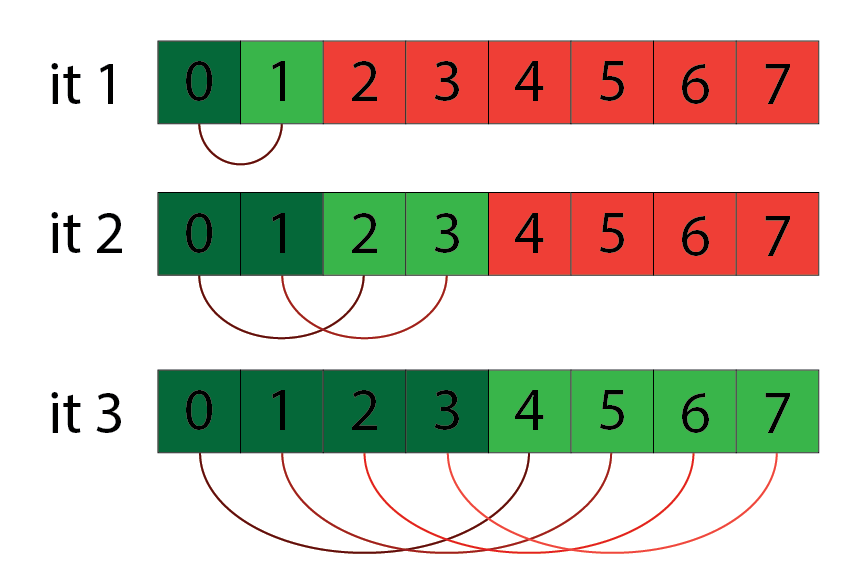
\includegraphics[width=\textwidth]{distribution}
    \caption{Iterations of the distribution of a message over 8 nodes.}
\end{figure}

From the above image one can clearly see that a problem occurs when the amount
of nodes is not a multiple of 2. For this reason the destination node is checked
to be smaller than the number of threads, so no invalid messages will be send.

\section{Discussion}
We are quite pleased with our solution, managing to maintain a complexity of
just $O(log(n))$ which means our program should run relatively fast even when
scaled to a much larger problem size. It did prove tricky to work out some of
the issues we had, for instance determining the destination nodes' ranks needed
some thought before we were able to come up with a solid way of doing this.

% =================================== REFERENCES ===================================

%\clearpage
%\bibliographystyle{unsrt}
%\bibliography{bib}

\end{document}
